% Skip over this boring header down a bit
%%%%%%%%%%%%%%%%%%%%%%%%%%%%%%%%%%%%%%%%%%%%%%%%
\documentclass[usenames,dvipsnames,10pt,aspectratio=169]{beamer} 
% Add option 'aspectratio=169' for 16:9 widescreen 
% Add option  'handout' to ignore animations
% If you have a smaller amount of text, feel free to also try '11pt'! / Jesper

\usepackage[utf8]{inputenc}
\usepackage{verbatim}
\usepackage{minted}
\usemintedstyle{monokai}
\usepackage{graphicx}
\usepackage{wrapfig}
\usepackage[document]{ragged2e}
\usetheme{umu}

\usepackage{hyperref}
\hypersetup{
    colorlinks=true,
    linkcolor=ucuyellow,
    filecolor=ucuyellow,      
    urlcolor=ucuyellow,
}
\urlstyle{same}

\usepackage[shortlabels]{enumitem}

%%% Bibliography
\usepackage[style=authoryear,backend=biber]{biblatex}
\addbibresource{bibliography.bib}

\DeclareNameAlias{author}{given-family}

%%% Suppress biblatex annoying warning
\usepackage{silence}
\WarningFilter{biblatex}{Patching footnotes failed}

%%% Some useful commands
% pdf-friendly newline in links
\newcommand{\pdfnewline}{\texorpdfstring{\newline}{ }} 
% Fill the vertical space in a slide (to put text at the bottom)
\newcommand{\framefill}{\vskip0pt plus 1filll}

%%% Enter additional packages below 
\renewcommand{\proofname}{\sffamily{Proof}}

%%%%%%%%%%%%%%%%%%%%%%%%%%%%%%%%%%%%%%%%%%%%%%%%%%%%%%%%%%%%%%%%%%%%%%%%%%%%%%%%%%%%%
\title[Rust \#3]{Rust \#3: Collections,\\ \vspace{0.1cm}
Iterators, and Traits}
\author[Sultanov Andriy]{Sultanov Andriy}
\institute{APPS@UCU}

\begin{document}

\begin{frame}
\titlepage
\end{frame}

\begin{frame}{\contentsname}
\tableofcontents
\end{frame}

\framepic{graphics/1.jpg}{
 \textcolor{ucuwhite}{Notes on inclusivity and safety}
 \vskip 0.5cm
 }

\section{Notes on inclusivity and safety}

\begin{frame}{Inclusivity}
	
\large
We've already talked about our responsibility as\\
programmers to use our powers to create good and\\
safe software. Tech isn't a goal of its own, it's a tool\\
(which we do enjoy using) to improve life for all of\\
humanity.\\

\vspace{0.3cm}

We haven't talked about different kind of responsibility,\\
responsibility inside of our own field, and especially\\
inside open source community. Tolerating sexism,\\
misogyny and outright abuse does not create safe and\\
inclusive spaces, and we should be rightly alarmed.

\end{frame}

\begin{frame}{Safety}

\large
Speaking about responsibility, Rust has a special\\
notion of \textcolor{ucuyellow}{safety/unsafety}. All the code we were\\
writing on these lectures before and will write\\
in the future is \textcolor{ucuyellow}{safe}, with all the constraints and\\
checks that Rust compiler imposes on us.\\

\vspace{0.3cm}

It is possible to skip those compiler checks, Rust\\
has a special "safety hatch" for that, a notion of\\
\textcolor{ucuyellow}{unsafety}, for which the programmer and not the\\
compiler should check semantic code correctness\\
and ensure that unsafe code is wrapped in safe APIs.\\
	
\end{frame}

\begin{frame}{Safety}
	
\large
Unsafe Rust allows you to:

\begin{itemize}[label=$\bullet$]
	\item Dereference raw pointers
	\item Call unsafe functions (including C functions, compiler intrinsics, and the raw allocator)
	\item Implement unsafe traits
	\item Mutate statics
	\item Access fields of unions
\end{itemize}

\end{frame}

\begin{frame}{Safety}
\vspace{0.3cm}
	\inputminted[fontsize=\large]{rust}{code/safety.rs}
\end{frame}

\framepic{graphics/1.jpg}{
 \textcolor{ucuwhite}{Collections in Rust}
 \vskip 0.5cm
 }

\section{Collections in Rust}

\begin{frame}{Collections}
	\framesubtitle{Most common collections}
	\large
	Rust's standard library implements some of\\
	the most common collections:
\begin{itemize}[label=$\bullet$]
	\item \textbf{Sequences}: \textcolor{ucuyellow}{String}, 
	\textcolor{ucuyellow}{Vec}, 
		\textcolor{ucuyellow}{VecDeque}, \textcolor{ucuyellow}{LinkedList}
	\item \textbf{Maps}: \textcolor{ucuyellow}{HashMap}, \textcolor{ucuyellow}{BTreeMap}
	\item \textbf{Sets}: \textcolor{ucuyellow}{HashSet}, \textcolor{ucuyellow}{BTreeSet}
	\item \textbf{Misc}: \textcolor{ucuyellow}{BinaryHeap}
\end{itemize}

	\vspace{0.4cm}
	In most cases, you are going to be fine with\\
	using just \textcolor{ucuyellow}{String}, \textcolor{ucuyellow}{Vec}, 
	\textcolor{ucuyellow}{HashMap}, \textcolor{ucuyellow}{HashSet}.
\end{frame}

\begin{frame}{Collections}
	\framesubtitle{String}
	\large
	Strings are dynamic (heap-allocated) UTF-8 collections!
	\vspace{0.3cm}
	\inputminted[fontsize=\large]{rust}{code/string.rs}
	\vspace{0.3cm}
\end{frame}

\begin{frame}{Collections}
	\framesubtitle{String}
	\large
	\inputminted[fontsize=\large]{rust}{code/string1.rs}
	\vspace{0.3cm}
\end{frame}

\begin{frame}{Collections}
	\framesubtitle{String}
	\large
	\inputminted[fontsize=\large]{rust}{code/string2.rs}
	\vspace{0.3cm}
\end{frame}

\begin{frame}{Collections}
	\framesubtitle{String}
	\large
	\inputminted[fontsize=\large]{rust}{code/string3.rs}
	\vspace{0.3cm}
\end{frame}

\begin{frame}{Collections}
	\framesubtitle{Vector}
	\large
	Vectors are your typical growable generic containers:
	\vspace{0.3cm}
	\inputminted[fontsize=\large]{rust}{code/vector.rs}
\end{frame}

\begin{frame}{Collections}
	\framesubtitle{Vector}
	\large
	\inputminted[fontsize=\normalsize]{rust}{code/vector1.rs}
	\vspace{0.3cm}
\end{frame}

\begin{frame}{Collections}
	\framesubtitle{HashMap}
	\large
	HashMap is a 'dictionary' type that's generic over <K, V>:
	\vspace{0.2cm}
	\inputminted[fontsize=\normalsize]{rust}{code/hashmap.rs}
\end{frame}

\begin{frame}{Collections}
	\framesubtitle{HashMap}
	\large
	\inputminted[fontsize=\large]{rust}{code/hashmap1.rs}
	\vspace{0.3cm}
\end{frame}

\begin{frame}{Collections}
	\framesubtitle{HashMap}
	\large
	\inputminted[fontsize=\Large]{rust}{code/hashmap2.rs}
	\vspace{0.3cm}
\end{frame}

\begin{frame}{Collections}
	\framesubtitle{HashSet}
	\large
	HashSet is a set that's generic over <T>:
	\vspace{0.2cm}
	\inputminted[fontsize=\normalsize]{rust}{code/hashset.rs}
\end{frame}

\begin{frame}{Collections}
	\framesubtitle{HashSet}
	\large
	\inputminted[fontsize=\large]{rust}{code/hashset1.rs}
\end{frame}

\framepic{graphics/1.jpg}{
	\textcolor{ucuwhite}{Generics and Traits}
 \vskip 0.5cm
 }

\section{Generics and Traits}

\begin{frame}{Generics}
	\framesubtitle{General}
	\Large
	Generics are a common way to generalize types and\\
	functionalities. This can reduce code duplication and\\
	allow for different and user-defined types to be\\
	used with generic functions.\\
	\vspace{0.4cm}
\end{frame}

\begin{frame}{Generics}
	\framesubtitle{Generic structs and enums}
	\large
	We've already seen a few examples of generic types\\
	in Rust (as opposed to concrete types): 
	\vspace{0.2cm}
	\inputminted[fontsize=\large]{rust}{code/generics1.rs}
\end{frame}

\begin{frame}{Generics}
	\framesubtitle{Generic structs and enums}
	Let's write one of these ourselves:
	\vspace{0.2cm}
	\inputminted[fontsize=\large]{rust}{code/generics2.rs}
\end{frame}

\begin{frame}{Generics}
	\framesubtitle{Generic structs and enums}
	\large
	We can also be more specific with \textcolor{ucuyellow}{impl} blocks:
	\vspace{0.2cm}
	\inputminted[fontsize=\large]{rust}{code/generics3.rs}
\end{frame}

\begin{frame}{Generics}
	\framesubtitle{Functions}
	\large
	In Rust, generics can be used in a lot of cases,\\
	let's first look at \textcolor{ucuyellow}{generic functions}.\\
	\vspace{0.2cm}
	Let's imagine we have two functions that are\\
	basically the same except for parameter types:\\
	\vspace{0.2cm}
	\inputminted[fontsize=\large]{rust}{code/generics4.rs}
\end{frame}

\begin{frame}{Generics}
	\framesubtitle{Functions}
	\large
	Let's rewrite these functions into a generic function:\\
	\vspace{0.2cm}
	\inputminted[fontsize=\Large]{rust}{code/generics5.rs}
	\vspace{0.2cm}
	This doesn't compile though...\\
\end{frame}

\begin{frame}{Traits}
	\framesubtitle{General}
	\large
	Rust, at compile-time, needs to be sure that you\\
	won't be able to call these functions with a type\\
	that won't have the needed functionality.\\
	\vspace{0.3cm}
	Rust has a concept that allows to tell the compiler\\
	about type's functionality, and to share that\\
	functionality between several types - \textcolor{ucuyellow}{traits}.\\
\end{frame}	

\begin{frame}{Traits}
	\framesubtitle{General}
	\large
	What's the type functionality? Basically - just the\\
	methods we can call on that type, and traits\\
	allow us to group those methods in specific sets.\\
	\vspace{0.4cm}
	Let's imagine we have several possible types of\\
	students - kindergarten, school and university\\
	students. We want to be able to get a report on\\
	them - with their names, grades etc.\\
\end{frame}

\begin{frame}{Traits}
	\framesubtitle{Example}
	\large
	We define an 'interface' of our shared functionality\\
	with method signatures without any implementation.\\
	We can also provide default functionality for a trait:\\
	\vspace{0.2cm}
	\inputminted[fontsize=\normalsize]{rust}{code/traits1.rs}
	\vspace{0.2cm}
\end{frame}

\begin{frame}{Traits}
	\framesubtitle{Example}
	\large
	Let's implement this trait for one of our student types:\\
	\vspace{0.2cm}
	\inputminted[fontsize=\normalsize]{rust}{code/traits2.rs}
\end{frame}

\begin{frame}{Traits}
	\framesubtitle{Traits as parameters}
	\large
	When we want to be sure that the type we take as a parameter\\
	has the needed functionality, we can use the \textcolor{ucuyellow}{impl Trait} syntax:\\
	\vspace{0.2cm}
	\inputminted[fontsize=\large]{rust}{code/traits3.rs}
\end{frame}

\begin{frame}{Traits}
	\framesubtitle{Traits as parameters}
	\large
	We can also specify having multiple traits\\
	implemented as a requirement:\\
	\vspace{0.2cm}
	\inputminted[fontsize=\large]{rust}{code/traits4.rs}
\end{frame}

\begin{frame}{Traits}
	\framesubtitle{Traits as parameters}
	\large
	If your function is generic over several types with\\
	different trait bounds, it's better to use \textcolor{ucuyellow}{where} syntax:\\	
	\vspace{0.2cm}
	\inputminted[fontsize=\large]{rust}{code/traits5.rs}
\end{frame}

\begin{frame}{Generics and Traits}
	\framesubtitle{Bounds}
	\large
	Let's return to an earlier example of a generic function:
	\vspace{0.2cm}
	\inputminted[fontsize=\Large]{rust}{code/generics5.rs}
	\vspace{0.2cm}
\end{frame}

\begin{frame}{Generics and Traits}
	\framesubtitle{Bounds}
	Why didn't it compile? Well, the compiler is actually quite helpful:\\
	\vspace{0.2cm}
	\inputminted[fontsize=\large]{rust}{code/generics6.rs}
\end{frame}

\begin{frame}{Generics and Traits}
	\framesubtitle{Bounds}
	\large
	Let's look at that \textcolor{ucuyellow}{std::ops::Add}:
	\vspace{0.2cm}
	\inputminted[fontsize=\large]{rust}{code/generics7.rs}
\end{frame}

\begin{frame}{Generics and Traits}
	\framesubtitle{Bounds}
	\large
	Let's add a bound on our generic function:\\
	\vspace{0.2cm}
	\inputminted[fontsize=\large]{rust}{code/generics8.rs}
	\vspace{0.6cm}
	But this doesn't compile, again...
\end{frame}

\begin{frame}{Generics and Traits}
	\framesubtitle{Bounds}
	\large
	Once again, Rust compiler saving our souls:
	\vspace{0.2cm}
	\inputminted[fontsize=\normalsize]{rust}{code/generics9.rs}
\end{frame}

\begin{frame}{Generics and Traits}
	\framesubtitle{Bounds}
	\large
	Alright, let's restrict it even further, now also\\
	considering that we don't want to borrow our\\
	arguments, we want to copy them:\\
	\vspace{0.2cm}
	\inputminted[fontsize=\large]{rust}{code/generics10.rs}
\end{frame}

\begin{frame}{Generics and Traits}
	\framesubtitle{std Traits}
	\large
	The standard library implements a lot of traits\\
	which allow it to reason about the functionality\\
	that certain types might have. The \textcolor{ucuyellow}{Copy} one\\
	we used	is a good example.\\
	\vspace{0.2cm}
	\inputminted[fontsize=\large]{rust}{code/traits6.rs}
	\vspace{0.2cm}
	This allows the Rust compiler to understand whether\\
	to move the object out or to copy it. 	
\end{frame}

\begin{frame}{Generics and Traits}
	\framesubtitle{std Traits}
	\large
	If the type implements a \textcolor{ucuyellow}{Copy} trait, it's usually just\\
	called Copy. For example, i32 is Copy, because it\\
	implements the trait and won't move out:\\
	\vspace{0.2cm}
	\inputminted[fontsize=\normalsize]{rust}{code/traits7.rs}
\end{frame}

\begin{frame}{Generics and Traits}
	\framesubtitle{std Traits}
	\large
	The standard library provides a lot of traits with default\\
	implementations which you can derive, among them:\\
	\vspace{0.2cm}
	\begin{itemize}[label=$\bullet$]
		\item \textbf{Debug} - Debug formatting using :?
		\item \textbf{PartialEq} and \textbf{Eq} - For $!=$ and $==$ implementations
		\item \textbf{PartialOrd} and \textbf{Ord} - For orderings using $<, >, <=, >=$
		\item \textbf{Hash} - Allows to map an instance to a value
	\end{itemize}
	\vspace{0.5cm}
	There are also 'marker' traits without any implementations,\\
	but they are beyond the scope of this lecture.\\
\end{frame}

\framepic{graphics/1.jpg}{
	\textcolor{ucuwhite}{Lifetimes}
 \vskip 0.5cm
 }

\section{Lifetimes}
\begin{frame}{Lifetimes}
	\large
	We've already talked about lifetimes a little, but so far\\
	we've mainly relied on the compiler to figure out lifetimes\\
	for us. Sometimes it's impossible for the compiler to\\
	reason about lifetimes, and we are forced to help it out.\\
	\vspace{0.4cm}
	This is where generic lifetimes come in. Yes, Rust has a lot\\
	of generic stuff - your functions can operate on generic\\
	types, 'generic' trait-implementing types and lifetimes.
\end{frame}

\begin{frame}{Lifetimes}
	\large
	Let's remind ourselves how Rust compiler\\
	reasons about lifetimes:\\
	\vspace{0.3cm}
	\inputminted[fontsize=\large]{rust}{code/lifetimes1.rs}
\end{frame}

\begin{frame}{Lifetimes}
	\large
	And now in the case of a simple function:
	\vspace{0.5cm}
	\inputminted[fontsize=\large]{rust}{code/lifetimes2.rs}
\end{frame}

\begin{frame}{Lifetimes}
	\large
	If the references do not contain explicit lifetime annotations,\\
	they are instead called implicit. We can write simple functions\\
	without explicitly annotating lifetimes of our parameters (just\\
	how we can omit types sometimes), and the function will be\\
	figured out by the compiler like this:\\
	\vspace{0.2cm}
	\inputminted[fontsize=\large]{rust}{code/lifetimes3.rs}
\end{frame}

\begin{frame}{Lifetimes}
	\large
	Generally, when it is possible, Rust compiler does not need\\
	our help and is able to figure out the lifetimes on its own.\\
	\vspace{0.4cm}
	It uses several rules for figuring out the lifetimes for functions:\\
	\begin{itemize}[label=$\bullet$]
		\item Each parameter that is a reference gets its own lifetime
		\item If there is one input lifetime, this lifetime is assigned\\
			to the return value
		\item If there are several input lifetimes, but one is \textcolor{ucuyellow}{self},\\
			its lifetime is assigned to the return value
	\end{itemize}
\end{frame}

\begin{frame}{Lifetimes}
	\large
	Let's try to apply these rules in a more complex case:
	\vspace{0.2cm}
	\inputminted[fontsize=\large]{rust}{code/lifetimes4.rs}
\end{frame}

\begin{frame}{Lifetimes}
	\large
	Rust compiler is not able to figure out the lifetime\\
	of the returned reference with these rules:
	\vspace{0.2cm}
	\inputminted[fontsize=\large]{rust}{code/lifetimes5.rs}
\end{frame}

\begin{frame}{Lifetimes}
	\large
	It will complain and try help us:
	\vspace{0.2cm}
	\inputminted[fontsize=\large]{rust}{code/lifetimes6.rs}
\end{frame}

\begin{frame}{Lifetimes}
	\large
	Let's introduce a single named lifetime parameter:
	\vspace{0.2cm}
	\inputminted[fontsize=\large]{rust}{code/lifetimes7.rs}
\end{frame}

\begin{frame}{Lifetimes}
	\large
	One special lifetime in Rust is \textcolor{ucuyellow}{'static}:
	\vspace{0.2cm}
	\inputminted[fontsize=\Large]{rust}{code/lifetimes8.rs}
	\vspace{0.2cm}
	It means that the reference will live for the entire\\
	duration of the program (indeed, string literals\\
	are just embedded into the program binary).\\
	\vspace{0.2cm}
	The compiler will often suggest you use this\\
	lifetime as an annotation, but you should only\\
	use it when it makes sense!
\end{frame}

\begin{frame}{Lifetimes}
	\large
	Rust functions can often get pretty messy when you use\\
	generic types, lifetimes and trait bounds:
	\vspace{0.2cm}
	\inputminted[fontsize=\large]{rust}{code/lifetimes9.rs}
\end{frame}

\framepic{graphics/1.jpg}{
	\textcolor{ucuwhite}{Iterators and Closures}
 \vskip 0.5cm
 }

\section{Iterators and Closures}

\begin{frame}{Closures}
	\large
	Closures are a common concept in functional programming,\\
	they are similar to lambda functions. In Rust, closures\\
	are anonymous inline functions which can be bound to\\
	variables. They are 'lazily' executed - will only start\\
	working when you call them.

	\vspace{0.5cm}
	\inputminted[fontsize=\Large]{rust}{code/closures1.rs}
\end{frame}

\begin{frame}{Closures}
	\large
	Rust will infer the types of closure parameters\\
	and return values, but we could include them\\
	explicitly, like in a function definition:\\
	\vspace{0.5cm}
	\inputminted[fontsize=\Large]{rust}{code/closures2.rs}
\end{frame}

\begin{frame}{Closures}
	\large
	Rust allows some variation with closures syntax,\\
	but they are still similar to functions:
	\vspace{0.5cm}
	\inputminted[fontsize=\Large]{rust}{code/closures3.rs}
\end{frame}

\begin{frame}{Closures}
	\large
	Why are they called closures? Because they 'close over'\\
	their environment, they can capture variables in their\\
	definition scope:\\
	\vspace{0.5cm}
	\inputminted[fontsize=\Large]{rust}{code/closures4.rs}
\end{frame}

\begin{frame}{Closures}
	\large
	Closures will figure out which variables they need and\\
	what they need to do with them, and will only borrow or\\
	move those. You should be aware of their behavior:\\
	\vspace{0.5cm}
	\inputminted[fontsize=\Large]{rust}{code/closures5.rs}
\end{frame}

\begin{frame}{Closures}
	\large
	You can force the closure to move the variables it needs.\\
	It might not actually take ownership of them if types are Copy!
	\vspace{0.5cm}
	\inputminted[fontsize=\Large]{rust}{code/closures6.rs}
	\vspace{0.5cm}
	This is often used with closures that run asynchronously\\
	and will need to survive longer than the current scope.
\end{frame}

\begin{frame}{Closures}
	\large
	Under the hood, closures are actually done using several traits:\\
	\vspace{0.5cm}
	\inputminted[fontsize=\large]{rust}{code/closures7.rs}
\end{frame}

\begin{frame}{Closures}
	\large
	So, your nice closure syntax will actually desugar to Rust\\
	creating a struct with all the variables you capture, and\\
	implementing the trait it needs on your struct.\\
	\vspace{0.5cm}
	Every closure is an \textcolor{ucuyellow}{FnOnce}, since it can be called once,\\
	closures that do not move their environment into them,\\
	but only borrow it mutably also are \textcolor{ucuyellow}{FnMut}, and closures\\
	that only borrow it immutably are also \textcolor{ucuyellow}{Fn}.\\
\end{frame}

\begin{frame}{Closures}
	\large
	You can take or return closures from functions using\\
	these traits as bounds:
	\vspace{0.3cm}
	\inputminted[fontsize=\large]{rust}{code/closures8.rs}
	\vspace{0.2cm}
	If you want to return closures, you will have to put them\\
	on the heap (since their size is not known at compile time)\\
	and move your environment into them.
	\vspace{0.2cm}
\end{frame}

\begin{frame}{Iterators}
	\large
	Iterators in Rust are not that different from your\\
	typical iterators in other languages. To be an Iterator\\
	you will have to implement an Iterator trait with a single\\
	required method:\\
	\vspace{0.3cm}
	\inputminted[fontsize=\large]{rust}{code/iterators1.rs}
	\vspace{0.3cm}
	Everything works thanks to Rust features: traits and\\
	algebraic types. While your iterator has values to return,\\
	it will return \textcolor{ucuyellow}{Some(Item)}, and once it runs out of them,\\
	it will start returning \textcolor{ucuyellow}{None}.
\end{frame}

\begin{frame}{Iterators}
	\large
	Everything works as you would expect:\\
	\vspace{0.3cm}
	\inputminted[fontsize=\large]{rust}{code/iterators2.rs}
\end{frame}

\begin{frame}{Iterators}
	\large
	You can also create mutable iterators, and iterators\\
	that will consume your collection:
	\vspace{0.3cm}
\begin{itemize}[label=$\bullet$]
	\item \textbf{.iter()} - iterates over \textcolor{ucuyellow}{\&T} \\
	\item \textbf{.iter\_mut()} - iterates over \textcolor{ucuyellow}{\&mut T}\\
	\item \textbf{.into\_iter()} - iterates over \textcolor{ucuyellow}{T}\\
\end{itemize}
\end{frame}

\begin{frame}{Iterators}
	Rust provides syntactic sugar for them:\\
	\vspace{0.3cm}
	\inputminted[fontsize=\Large]{rust}{code/iterators3.rs}
\end{frame}

\begin{frame}{Iterators}
	\inputminted[fontsize=\Large]{rust}{code/iterators4.rs}
\end{frame}

\begin{frame}{Iterators}
	\inputminted[fontsize=\Large]{rust}{code/iterators5.rs}
\end{frame}

\begin{frame}{Iterators}
	\large
	Once you implement the .next() method, you will get default\\
	implementations of a lot of adapters:\\
	\vspace{0.3cm}
	\inputminted[fontsize=\normalsize]{rust}{code/iterators6.rs}
	\vspace{0.3cm}
\end{frame}

\begin{frame}{Iterators}
	\large
	Rust's iterators are heavily optimized, so you shouldn't\\
	feel bad about using a bunch of adapters one over another.\\
	\vspace{0.3cm}
	They are essential for idiomatic collection processing,\\
	and you should spend some time looking over their official\\
	documentation and learn which adapters you need!
\end{frame}
 
\framepic{graphics/1.jpg}{
	\textcolor{ucuwhite}{Thank you!}
 \vskip 0.5cm
 }

%\begin{frame}{Resources}
	%\Large
	%\begin{figure}[c]
		%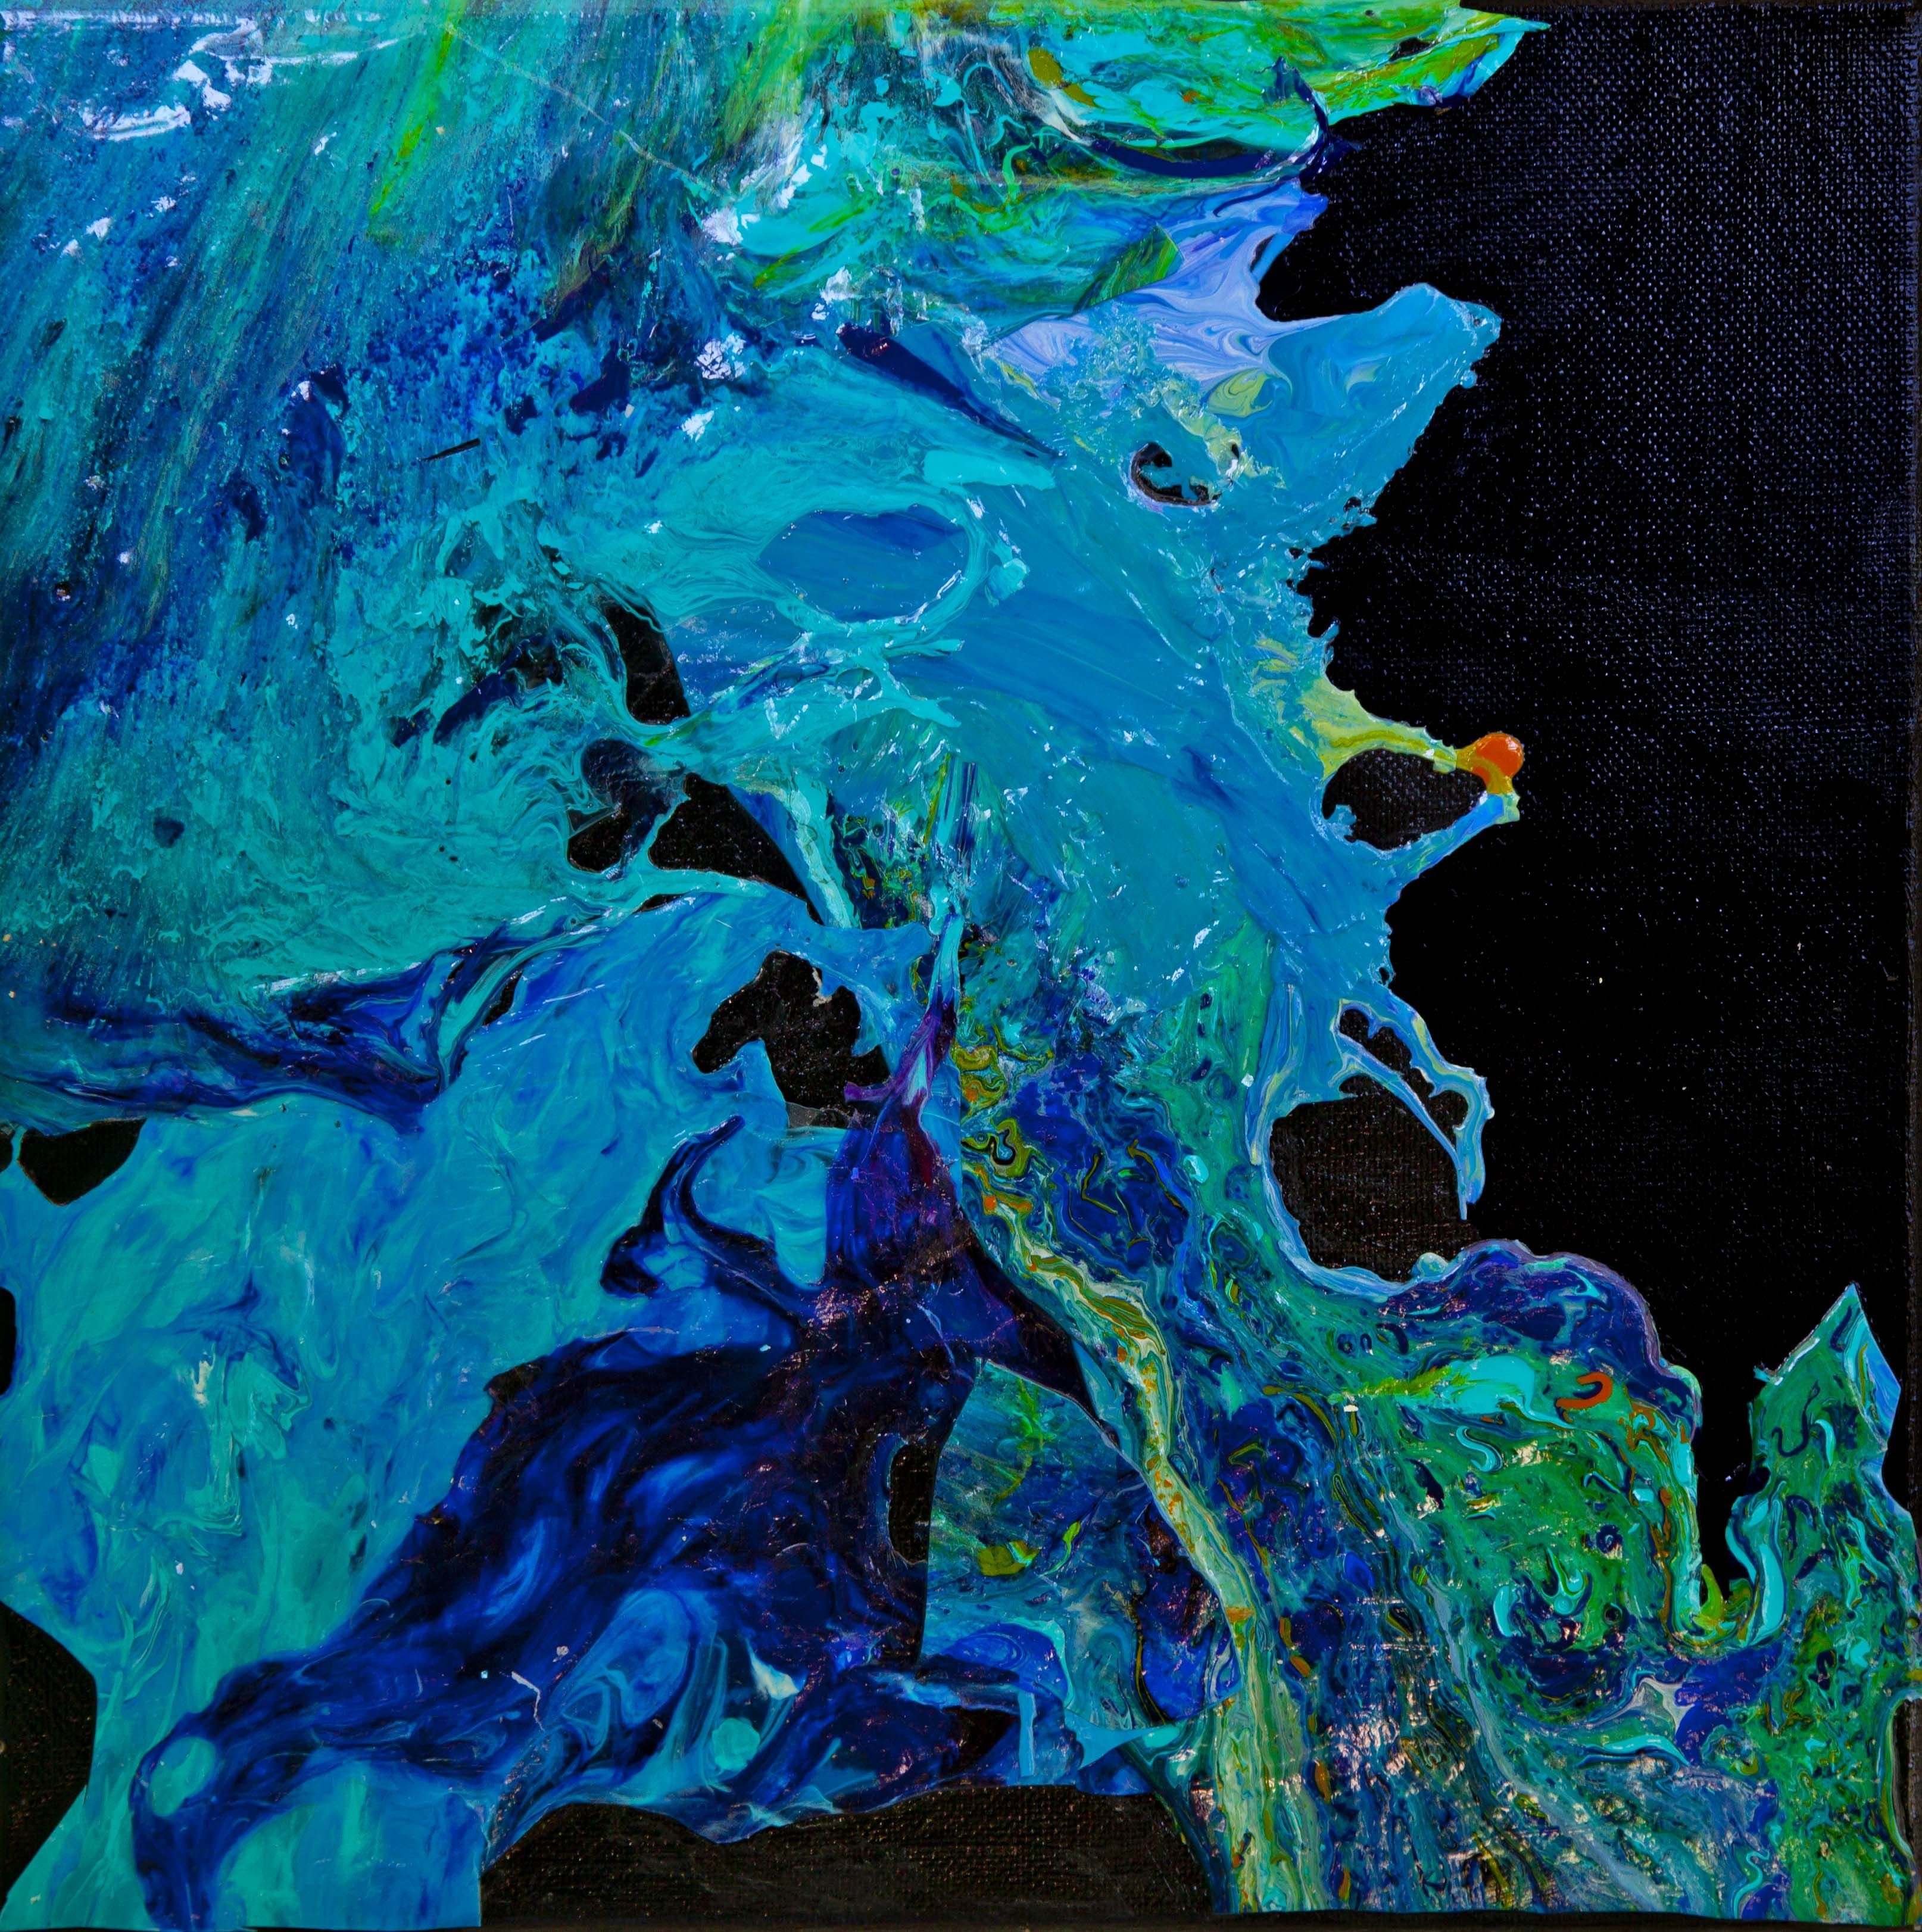
\includegraphics[width=1\linewidth]{graphics/1.jpg}
	%\end{figure}
%\end{frame}

\end{document}
